\documentclass[a4paper, 12pt]{article}

\usepackage{geometry}
\usepackage{amsmath}
\usepackage{gvv}

\title{Question 7.4.7}
\author{AI25BTECH11040 - Vivaan Parashar}
\date{\today}

\begin{document}

\maketitle

\section{Question: }
The intercept of the line $y = x$ by the circle $x^2 + y^2 - 2x = 0$ is $AB$. Equation of the circle with $AB$ as a diameter is \underline{\hspace{2cm}}.

\section{Solution: }
Let's assume the two points, $\vec{A}$ and $\vec{B}$, where the line $y = x$ intersects the circle $x^2 + y^2 - 2x = 0$.
The two points lie on the line, whose equation can be expressed in matrix form as:
\begin{align}
    \myvec{1 \\ -1}^\mathrm{T}\vec{x} = 0
\end{align}
Therefore, we have:
\begin{align}
    \myvec{1          & -1}\vec{A} = 0                               \\
    \myvec{1          & -1}\vec{B} = 0                               \\
    \implies \myvec{1 & -1}\myvec{\vec{A} & \vec{B}} = \myvec{0 & 0}
\end{align}
We also have the equation of the circle in the matrix form as:
\begin{align}
    \norm{\vec{x}}^2 + 2\vec{u}^\mathrm{T}\vec{x} + f = 0 \\
    \text{where, } \vec{u} = -\vec{O}, f = \norm{\vec{O}}^2 - r^2
\end{align}
Here, $\vec{O}$ is the center of the circle and $r$ is its radius. Comparing the given equation of the circle ($(x-1)^2+y^2=1$) with the above equation, we get:
\begin{align}
    \vec{O} = \myvec{1 \\ 0}, r = 1
\end{align}
Thus, we have the equation of the circle as:
\begin{align}
    \vec{u} = \myvec{-1 \\ 0}, f = 0\\
    \implies \norm{\vec{x}}^2 - 2\myvec{1 & 0}\vec{x} = 0
\end{align}
Since both points $\vec{A}$ and $\vec{B}$ lie on the circle, we have:
\begin{align}
    \norm{\vec{A}}^2 - 2\myvec{1 & 0}\vec{A} = 0 \\
    \norm{\vec{B}}^2 - 2\myvec{1 & 0}\vec{B} = 0 \\
    \implies \myvec{\vec{A} & \vec{B}}^\mathrm{T}\myvec{\vec{A} & \vec{B}} - 2\myvec{1 & 0}\myvec{\vec{A} & \vec{B}} = \myvec{0 & 0}
\end{align}

\section{Plot: }
\begin{figure}[h!]
    \centering
    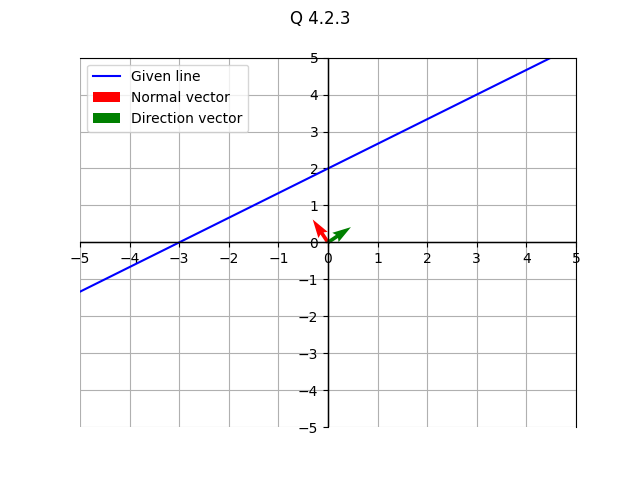
\includegraphics[width=\columnwidth]{figs/plot.png}
    \caption{Graph of line with direction and normal vectors}
    \label{fig:7.4.7}
\end{figure}


\end{document}